\section{Scopo e strumentazione}

Nel corso dell'esperienza sfrutteremo un OpAmp (TL081) per realizzare circuiti non lineari, valutandone di volta in volta le caratteristiche e i limiti di funzionamento.

\section{Discriminatore}

\begin{figure}[h]
	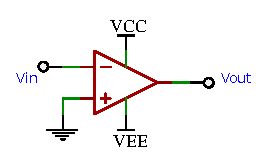
\includegraphics{circ_discr.pdf}
	\caption{Circuito Discriminatore}
	\label{f:discr}
\end{figure}

Si è montato il circuito come in \fig{discr}, inviando segnali sinusoidali in ingresso. La normale risposta del circuito può essere osservata in \fig{discr_normale}: di fatto, il segnale 

\begin{figure}
	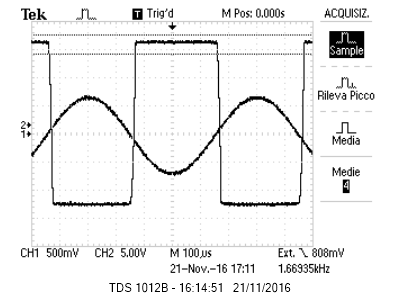
\includegraphics{risposta_normale_1.png}
	\caption{Risposta del discriminatore ad un segnale sinusoidale}
	\label{f:discr_normale}
\end{figure}
